\chapter{Adminsitración}
\label{capadministracion}

La capa de Administración de VirtShell proporciona una infraestructura de servicios para la gestión de cualquier dispositivo registrado y creado a traves del sistema. Este capítulo busca darle explicación a las funcionalidades de administración para utilizarlas en su beneficio.

\section{Particiones, anfitriones y Ambientes en VirtShell}
En VirtShell hay tres conceptos que son muy importantes y se extiende a través de todos los servicios, y que simplemente no puede dejar de tener en cuenta: Las particiones, los ambientes y las instancias. Las tres se asocian con la mayoría de las cosas en VirtShell, y el dominio de ellos es crucial para una buena administración de los dispositivos. 

\subsection{Particiones}
Las particiones consisten de uno o más anfitriones, los cuales pueden ser nodos físicos, servidores o incluso máquinas virtuales. El objetivo principal que busca una partición, es organizar las máquinas que albergaran recursos virtuales en partes aisladas de las demás. Estas partes pueden pueden estar ubicadas en un mismo sitio físico o por el contrario puede estar distribuidas es diferentes zonas geográficas de todo el mundo.\\
\\
Si solo se cuenta con un numero fijo de maquinas (o anfitriones) ubicadas en un mismo sitio físico como por ejemplo un datacenter \footnote{Un data center también llamado centro de datos es un espacio acondicionado especialmente para contener a todos los equipos y sistemas de TI}, lo que se obtiene con las particiones es la posibilidad de dividir esas maquinas en subgrupos que puedan ser destinados para diferentes equipos o divisiones dentro de una organización.\\ 
\\
Al contar con maquinas distribuidas en diferentes zonas geográficas la elección de una partición u otra se basa principalmente en la cercanía de los visitantes o clientes, ya que a menor distancia entre los servidores y ellos, menores son los tiempos de respuesta y mejor la experiencia de usuario.\\
\\
Las particiones también favorecen la disponibilidad. Si distribuye sus instancias a través de múltiples particiones y una instancia falla, puede diseñar su aplicación para que una instancia en otra partición pueda atender las peticiones.\\
\\
Cuando se crea una nueva partición, VirtShell la crea completamente vaciá, sin anfitriones. Para asociar anfitriones a una partición se debe crear un anfitrión y vincularlo con la partición como se vera mas adelante en este mismo capítulo. Un ejemplo de como crear una partición usando el API se muestra en el siguiente código:

\begin{lstlisting}[style=json, caption=Petición HTTP para crear una partición]
curl -sv -X POST \
  -H 'accept: application/json' \
  -H 'X-VirtShell-Authorization: UserId:Signature' \
  -d '{
       "name": "development_co",
       "description": "Collection of servers oriented to development team in colombia."
      }' \
   'http://localhost:8080/api/virtshell/v1/partitions'
\end{lstlisting}


\subsection{Asociación de anfitriones a particiones}
Los anfitriones no son mas que nodos físicos, servidores o máquinas virtuales, que alojaran recursos virtuales. VirtShell ofrece la posibilidad de clasificarlos de acuerdo a combinaciones de capacidad de CPU, memoria, almacenamiento y red. El objetivo que busca la clasificación es proporcionar flexibilidad para elegir la combinación de recursos adecuada para las aplicaciones.\\
\\
Los tipos de anfitriones se agrupan en familias basadas en perfiles de aplicación de destino. Estos grupos incluyen: de propósito general, con procesadores de alto desempeño, de memoria optimizada, de almacenamiento optimizado.

\begin{description}
\item [Propósito general] Esta familia proporciona un equilibrio de recursos informáticos, de memoria y red, por lo que constituye una buena opción para muchas aplicaciones.
\item [Procesadores de alto desempeño] Esta familia ofrece procesadores que alcanzan alto desempeño en tareas complejas.
\item [Memoria optimizada] Esta familia esta optimizada para aplicaciones con un uso intenso de la memoria.
\item [Almacenamiento optimizado] Esta familia promete anfitriones con alta capacidad de almacenamiento, optimizado para un desempeño de E/S muy alto.
\end{description}

Cuando se crea un anfitrión en VirtShell este debe ser asociado a una sola partición, asignándole un tipo, con alguno de los mencionados anteriormente, estableciendo las capacidad de disco y memoria RAM con las que cuenta,  
indicando también el sistema operativo y las ip con las que se conecta a la red. Una vez el anfitrión es creado en el sistema este queda asignado a la partición elegida. El siguiente ejemplo muestra como crear un anfitrión usando el API:

\begin{lstlisting}[style=json, caption=Petición HTTP para crear un host]
curl -sv -X POST \
  -H 'accept: application/json' \
    -H 'X-VirtShell-Authorization: UserId:Signature' \
  -d '{"name": "host-01-pdn",
       "os": "Ubuntu_12.04_3.5.0-23.x86_64",
       "memory": "16GB",
       "capacity": "120GB",
       "enabled": "true",
       "type" : "GeneralPurpose",
       "local_ipv4": "15.54.88.19",
       "local_ipv6": "ff06:0:0:0:0:0:0:c3",
       "public_ipv4": "10.54.88.19",
       "public_ipv6": "yt06:0:0:0:0:0:0:c3",
       "partition": "development_co"}' \
   'http://localhost:8080/virtshell/api/v1/hosts'
\end{lstlisting}

\vspace{5mm}

En este ejemplo se muestra la creación de un anfitrión con nombre host-01-pdn que esta clasificado como de uso general y que queda asociado a la partición development\_co creada en la sección anterior.\\
\\
Al consultar la partición nuevamente por medio del API se puede observar como el anfitrión se encuentra asociado a la partición developtment\_co. En la siguiente consulta al API se muestra el resultado de la asociación:

\vspace{5mm} 

\begin{lstlisting}[style=json, , caption=Petición HTTP para consultar una partición por su nombre]
curl -sv -H 'accept: application/json' 
     -H 'X-VirtShell-Authorization: UserId:Signature' \ 
     'http://<host>:<port>/api/virtshell/v1/partitions/development_co'
\end{lstlisting}

\vspace{5mm}

Respuesta:

\vspace{5mm}

\begin{lstlisting}[style=json]
HTTP/1.1 200 OK
Content-Type: application/json
{
  "uuid": "efa1777c-cad7-11e5-9956-625662870761",
  "name": "development_co",
  "description": "Collection of servers oriented to development team in colombia.", 
  "hosts": [ "host-01-pdn" ],  
  "created": {"at":"1429207233", 
              "by":"1a900cdc-cad8-11e5-9956-625662870761"}
}
\end{lstlisting}

\vspace{5mm}

Adicionalmente, cuando un anfitrión es agregado a una partición, VirtShell instala automáticamente los agentes  que realizaran tareas de aprovisionamiento y monitoreo. Los agentes se explicaran mas adelante.

\subsection{División de particiones en ambientes}
Las particiones se refieren a la forma de organizar lugares físicos. Los ambientes por el contrario, son lugares lógicos y aislados dentro de una partición. Cada partición puede estar compuesta por uno o varios ambientes, y un ambiente puede contener uno o mas instancias. Cada ambiente pertenece a una sola partición. La figura \ref{fig:enviroment} muestra un ejemplo de como dos particiones contiene varios ambientes destinados a equipos de trabajo diferentes. \\

\begin{figure}[h]
    \centering
  \caption{Ejemplo de ambientes en un partición}
  \label{fig:enviroment}
  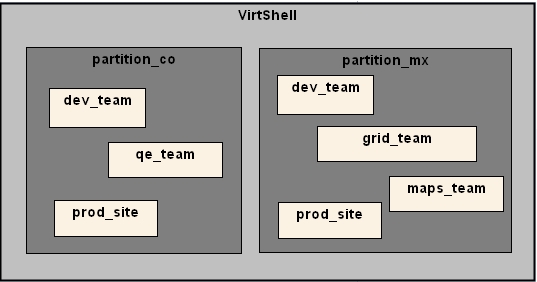
\includegraphics[width = 0.95\textwidth]{../architecture/v1/diagrams/enviroments}
\end{figure}

Un ejemplo de como crear un ambiente asociado a una partición usando el API se muestra en el siguiente código:

\begin{lstlisting}[style=json, caption=Petición HTTP para crear un ambiente]
curl -sv -X POST \
  -H 'accept: application/json' \
  -H 'X-VirtShell-Authorization: UserId:Signature' \
  -d '{
       "name": "bigdata_laboratory",
       "description": "Collection of servers oriented to big data.", 
       "partition": "bogota_partition_co"
      }' \
   'http://localhost:8080/api/virtshell/v1/enviroments'
\end{lstlisting}

\section{Instancias}
A un servidor virtual en VirtShell, se le denomina instancia, las cuales pueden ser maquinas virtuales que corren sobre algún hipervisor o también pueden ser contenedores que se ejecutan directamente sobre el sistema operativo del anfitrión. \\
\\
La elección de la tecnología de virtualización depende de las preferencias u objetivos que se busque con las aplicaciones de la instancia. En la actualidad VirtShell soporta Virtualbox como hipervisor para maquinas virtuales y para los contenedores soporta LXC \footnote{LXC (Linux Containers) es una tecnología de virtualización en el nivel de sistema operativo (SO) para Linux. } \cite{lxc16} y Docker \footnote{Docker es un proyecto de código abierto que automatiza el despliegue de aplicaciones dentro de contenedores de software, proporcionando una capa adicional de abstracción y automatización de Virtualización a nivel de sistema operativo en Linux.} \cite{docker16}.\\
\\
Las instancias son designadas a solo ambiente de trabajo en el momento de ser creadas. En el instante de su creación, se debe especificar las características de CPU, memoria y capacidad de disco que se desea. De igual manera, se configura el sistema operativo, los permisos para los demás usuarios del sistema, el tipo de anfitrión que necesita y la tecnología que se desea usar para virtualizar.

\subsection{Creación de instancias en un ambiente}
Cuando se recibe una solicitud de creación de una instancia, VirtShell selecciona un anfitrión, de los que se encuentran configurados en la partición a la cual pertenece el ambiente donde se quiere crear la instancia. En la solicitud de creación se debe especificar el tipo de anfitrión que se requiere para el correcto funcionamiento de las aplicaciones que se ejecutaran ahí. Si la partición no cuenta con el tipo de anfitrión solicitado, se rechazara la petición detallando el inconveniente. Si por el contrario la selección del anfitrión es exitosa, VirtShell procede a enviar la solicitud al agente de aprovisionamiento del anfitrión escogido. \\
\\
Debido a que una solicitud de aprovisionamiento puede involucrar mas de una instancia, el servidor de VirtShell responde la solicitud de aprovisionamiento con el estado de \emph{in-progress} (en progreso) y a su vez con el identificador de una tarea. La tarea será ejecutada de manera asincrónica y el usuario por medio del API REST puede consultar el estado y avance de la misma (Las tareas se ampliaran en la siguiente sección).\\
\\
Un ejemplo de la creación de una instancia usando el API se muestra en el siguiente código:

\begin{lstlisting}[style=json, caption=Petición HTTP para crear una instancia]
curl -sv -X POST \
  -H 'accept: application/json' \
  -H 'X-VirtShell-Authorization: UserId:Signature' \
  -d '{ "name": "transactional_log",
        "memory": 8024,
        "cpus": 2,
        "hdsize": "20GB",
        "enviroment": "development_co",
        "operating_system": "ubuntu_server_14.04.2_amd64",
        "description": "Server transactional only for store logs", 
        "provisioner": "all_backend",
        "host_type": "GeneralPurpose",
        "driver": "lxc"
      }' \
   'http://localhost:8080/api/virtshell/v1/instances'
\end{lstlisting}

\vspace{5mm}

En esta solicitud HTTP se observa que la instancia a crear debe tener el  sistema operativo es Linux Ubuntu, contar con 8 Gigabytes de memoria RAM, dos núcleos, 20 Gigabyte de disco duro, y que debe ser creada en el ambiente de nombre development\_co en una maquina física de uso general. Adicionalmente la instancia debe ser un contenedor que se ejecute sobre LXC.\\
\\
Si la solicitud de las características es exitosa, el servidor responderá de la siguiente manera:

\vspace{5mm}

\begin{lstlisting}[style=json, caption=Ejemplo de respuesta HTTP a la solicitud de crear una instancia]
HTTP/1.1 200 OK
Content-Type: application/json
{ "create": "in progress", "task": "bbf6669b-1b83-4fe7-ae2a-2b31738c4165" }
\end{lstlisting}

Si por el contrario, la solicitud no es exitosa, el servidor responderá con el respectivo código de error HTTP y la razón por la cual no se pudo procesar exitosamente la petición. Un ejemplo de una petición no procesada es la siguiente: 

\vspace{5mm}

\begin{lstlisting}[style=json, caption=Ejemplo de respuesta HTTP con error a la solicitud de crear una instancia]
HTTP/1.1 500 OK
Content-Type: application/json
{ "create": "error", "reason": "The enviroment doesn't have the host_type requested" }
\end{lstlisting}

\vspace{5mm}

Adicional a la creación de instancias, el API REST de VirtShell proporciona URIs para su gestión. Las operaciones sobre el ciclo de vida de una instancia que permite realizar son: iniciar, detener, reiniciar, cerrar y clonar. Así mismo, el API posibilita la fácil y rápida búsqueda de una o mas instancias.  

\section{Tareas}
Una tarea es una actividad asincrónica, que se ejecuta en \emph{background} (segundo plano), y se crea de manera automática cuando se solicita una acción al servidor, y esta pueda tomar un largo periodo de tiempo para completar su trabajo.\\
\\
Las tareas asíncronas resuelven los problemas relacionados con los tiempos de espera de las conexiones, los tiempos de espera de la solicitudes o los tiempos de vida de las peticiones HTTP antes de que estas sean cerradas por el servidor de aplicaciones web o por el navegador de manera automática de acuerdo a sus parámetros de configuración.\\
\\
Las operaciones de larga duración en VirtShell son las que involucran acciones en las instancias. Debido a que estas ultimas pueden estar físicamente lejanas del servidor, el tiempo de espera de una petición HTTP puede incrementarse lo suficiente para que esta sea finalizada por el servidor web. Asimismo, las operaciones de aprovisionamiento de las instancias, las cuales consisten principalmente en instalación y configuración de paquetes son tareas que involucran componentes realizados por terceros sobre los cuales no se tiene control sobre sus tiempos de respuesta.\\
\\
Cuando VirtShell recibe una petición y esta es considerada de larga duración, en el cuerpo de la respuesta se enviá la acción recibida con el estado de \emph{in progress} acompañado del identificador único UUID \footnote{UUID son las siglas en inglés del Identificador Universalmente Único.} de la tarea. Por ejemplo, si se recibe una petición de instalación de un paquete en una o mas instancias, la respuesta HTTP seria de la siguiente forma:

\begin{lstlisting}[style=json, caption=Ejemplo de respuesta HTTP referenciando a una tarea]
HTTP/1.1 200 OK
Content-Type: application/json
{ "install-package": "in progress", "task": "908b4d78-8b7a-40d7-9ecf-5036eeb5526b" }
\end{lstlisting}

\vspace{5mm}

Para consultar por el estado de una tarea, se invoca el API de VirtShell, enviando en la url, el identificador UUID recibido de la primera petición, el servidor responderá con un documento en formato JSON detallando la tarea y su estado. El siguiente es un ejemplo de una consulta sobre una tarea y la respuesta del servidor:

\vspace{5mm}

\begin{lstlisting}[style=json, caption=Ejemplo de consulta de una tarea]
curl -sv -H 'accept: application/json' 
     -H 'X-VirtShell-Authorization: UserId:Signature' \ 
     'http://<host>:<port>/api/virtshell/v1/tasks/908b4d78-8b7a-40d7-9ecf-5036eeb5526b'
\end{lstlisting}

\vspace{5mm}

Respuesta:

\vspace{5mm}


\begin{lstlisting}[style=json, caption=Ejemplo del detalle de una tarea]
HTTP/1.1 200 OK
Content-Type: application/json
```
```json
{
  "uuid": "908b4d78-8b7a-40d7-9ecf-5036eeb5526b",
  "description": "install-package in instance database_01",
  "status" : "installing",
  "created": {"at":"1429207233", "by":"92d30f0c-8c9c-11e5-8994-feff819cdc9f"},
  "last_update": "1429207435",
  "log": "installing package couchdb"
}
\end{lstlisting}


\section{Propiedades}
Las propiedades sirven para obtener información de las instancias y anfitriones. Por medio de ellas se pueden conocer características de configuración de red, cantidad de memoria en uso, porcentaje de procesador usado en un determinado momento, numero de procesos en ejecución y una gran variedad de información útil del sistema.\\
\\
Las propiedades pueden ser consultadas para una o mas instancias al mismo tiempo, definiendo el nombre de cada una de ellas. También pueden ser consultadas varias características del sistema al mismo tiempo. El siguiente ejemplo muestra la forma de consultar varias propiedades de una instancia:

\vspace{5mm}


\begin{lstlisting}[style=json, caption=Ejemplo consultando varias propiedades a una instancia]
curl -sv -X GET \
  -H 'accept: application/json' \
  -H "Content-Type: text/plain" \
  -H 'X-VirtShell-Authorization: UserId:Signature' \
  -d '{ "properties": [{"name": "memory"}, {"name": "cpu"}],
        "hosts": [{"name": "WebServer001"}]}' \
   'http://localhost:8080/api/virtshell/v1/properties'
\end{lstlisting}


\vspace{5mm}

Respuesta:

\begin{lstlisting}[style=json, caption=Respuesta]
HTTP/1.1 200 OK
Content-Type: application/json
```
```json
{
  "name": "WebServer001",
  "memory": 8024,
  "cpu": 87.4
}
\end{lstlisting}


\vspace{5mm}

En el segundo ejemplo se muestra la forma de consultar varias propiedades a una o mas instancias:

\vspace{5mm}

\begin{lstlisting}[style=json, caption=Ejemplo consultando propiedades a varias instancias]
curl -sv -X GET \
  -H 'accept: application/json' \
  -H "Content-Type: text/plain" \
  -H 'X-VirtShell-Authorization: UserId:Signature' \
  -d '{ "properties": [{"name": "memory"}, {"name": "cpu"}],
        {"name": "Database00", "range": "[1-3]"}]}' \
   'http://localhost:8080/api/virtshell/v1/properties'
\end{lstlisting}

\vspace{5mm}

Respuesta:

\begin{lstlisting}[style=json, caption=Respuesta]
HTTP/1.1 200 OK
Content-Type: application/json
```
```json
{
  properties: [
    {
     "id": "kj5436c0-dc94-13tg-82ce-9992b5d5c51b",
     "name": "Database001",
     "memory": 4024,
     "cpu": 2
    },
    {
     "id": "591b3828-7aaf-4833-a94c-ad0df44d59a4",
     "name": "Database002",
     "memory": 4024,
     "cpu": 1  
    },
    {
     "id": "f7c81039-5c88-423b-8b0d-c124483d586b",
     "name": "Database003",
     "memory": 4024,
     "cpu": 3  
    }
  ]  
}
\end{lstlisting}